\documentclass[conference]{IEEEtran}
\IEEEoverridecommandlockouts
%Template version as of 6/27/2024

\usepackage[utf8]{inputenc}
\usepackage[spanish,es-tabla,es-nodecimaldot]{babel}
\usepackage{cite}
\usepackage{amsmath,amssymb,amsfonts}
\usepackage{algorithmic}
\usepackage{graphicx}
\usepackage{textcomp}
\usepackage{xcolor}
\usepackage{verbatim}
\usepackage{booktabs}
\usepackage{multirow}
\usepackage{siunitx}
\newcommand{\TODO}[1]{\textcolor{red}{\textbf{TODO: #1}}}
% Auto-generated LaTeX macros from results/benchmarks_summary.csv
\newcommand{\macrocputputscalar}{0.11}
\newcommand{\macrocpuenergyscalarnet}{45.58}
\newcommand{\macrocpuenergyscalargross}{92.72}
\newcommand{\macrocpuenergyscalarpower}{10.1}
\newcommand{\macrocpuenergyscalarpowers}{10.1~W}
\newcommand{\macrocputputshani}{0.89}
\newcommand{\macrocpuenergyshaninet}{5.28}
\newcommand{\macrocputputtwo}{1.78}
\newcommand{\macrocpuenergytwonet}{4.47}
\newcommand{\macrocputputfour}{3.55}
\newcommand{\macrocpuenergyfournet}{4.13}
\newcommand{\macrocpuenergyfournets}{4.13~J/GB}
\newcommand{\macrocpuenergyfourgross}{5.58}
\newcommand{\macrocpuenergyfourgrosss}{5.58~J/GB}
\newcommand{\macrocpuenergyfourpower}{19.8}
\newcommand{\macrocpuenergyfourpowers}{19.8~W}
\newcommand{\macrocputputeight}{5.60}
\newcommand{\macrocpuenergyeightnet}{2.67}
\newcommand{\macrocpuenergyeightpower}{20.1}
\newcommand{\macrocputputtwelve}{5.62}
\newcommand{\macrocpuenergytwelvenet}{2.69}
\newcommand{\macrocpuenergytwelvenets}{2.69~J/GB}
\newcommand{\macrocpuenergytwelvegross}{3.61}
\newcommand{\macrocpuenergytwelvegrosss}{3.61~J/GB}
\newcommand{\macrocpuenergytwelvepower}{20.3}
\newcommand{\macrocpuenergytwelvepowers}{20.3~W}
\newcommand{\macrocputputtwelvepe}{5.84}
\newcommand{\macrocpuenergytwelvepenet}{2.53}
\newcommand{\macrocpuenergytwelvepenets}{2.53~J/GB}
\newcommand{\macrogputputkernel}{15.62}
\newcommand{\macrogpuenergykernelnet}{1.62}
\newcommand{\macrogpuenergykernelgross}{1.90}
\newcommand{\macrogpupowerkernel}{29.7}
\newcommand{\macrogpupowerkernelw}{29.7~W}
\newcommand{\macrogpuenergykernelnets}{1.62~J/GB}
\newcommand{\macrogpuenergykernelgrosss}{1.90~J/GB}
\newcommand{\macrogpuenergykernelconhost}{2.45}
\newcommand{\macrogpuenergykernelconhosts}{2.45~J/GB}
\newcommand{\macrogputputeetwopinned}{4.98}
\newcommand{\macrogpuenergyeetwonet}{3.49}
\newcommand{\macrogpuenergyeetwogross}{4.38}
\newcommand{\macrogpupowereetwo}{21.8}
\newcommand{\macrogpupowereetwow}{21.8~W}
\newcommand{\macrogpuenergyeetwonets}{3.49~J/GB}
\newcommand{\macrogpuenergyeetwogrosss}{4.38~J/GB}
\newcommand{\macrogpuenergyeetwoconhost}{5.48}
\newcommand{\macrogpuenergyeetwoconhosts}{5.48~J/GB}
\newcommand{\macrogputputeetwopageable}{3.86}
\newcommand{\macrogpuenergyeetwopageablenets}{3.77~J/GB}
\newcommand{\macrogpuenergyeetwopageableconhosts}{6.34~J/GB}
\newcommand{\macrogpupeakkernel}{22.29}
\newcommand{\macrogpupeakeetwo}{5.87}
\newcommand{\macrocpuenergyidlepower}{5.15}
\newcommand{\macrocpuenergyidlepowers}{5.15~W}
\newcommand{\macrogpupoweridle}{4.44}
\newcommand{\macrogpupoweridles}{4.44~W}

\def\BibTeX{{\rm B\kern-.05em{\sc i\kern-.025em b}\kern-.08em
    T\kern-.1667em\lower.7ex\hbox{E}\kern-.125emX}}
\begin{document}

\title{Desarrollo y evaluación de un Acelerador Criptográfico para el Algoritmo SHA-2 en Hardware Reconfigurable\\
}

\author{\IEEEauthorblockN{1\textsuperscript{st} Benjamín Oyarzún Valdebenito}
\IEEEauthorblockA{\textit{Departamento de Ingeniería Eléctrica} \\
\textit{Universidad de Santiago de Chile}\\
Santiago, Chile \\
benjamin.oyarzun.v@usach.cl}
\and
\IEEEauthorblockN{2\textsuperscript{nd} Nicolás Ruminot Ahumada}
\IEEEauthorblockA{\textit{Departamento de Ingeniería Eléctrica} \\
\textit{Universidad de Santiago de Chile}\\
Santiago, Chile \\
nicolas.ruminot@usach.cl}
\and
\IEEEauthorblockN{3\textsuperscript{rd} Christian Fernández-Campusano}
\IEEEauthorblockA{\textit{Departamento de Ingeniería Eléctrica} \\
\textit{Universidad de Santiago de Chile}\\
Santiago, Chile \\
christian.fernandez@usach.cl}
}

\maketitle

\begin{abstract}
El algoritmo criptográfico SHA-256 es fundamental en la seguridad de redes y en sistemas de consenso distribuido, donde la constante validación de bloques impone una elevada demanda computacional y energética. Este articulo presenta un análisis comparativo y experimental de dicho algoritmo sobre tres arquitecturas heterogéneas: un procesador multinúcleo Intel Core i7 con extensiones vectoriales SHA-NI, un acelerador gráfico masivamente paralelo NVIDIA GeForce RTX 2050 y un coprocesador dedicado desarrollado en Verilog RTL sobre una tarjeta FPGA AMD Spartan-7. A diferencia de estudios previos enfocados en minería sintética de un único bloque, la evaluación emplea una carga de trabajo homogénea de un gigabyte dividida en millones de mensajes independientes de sesenta y cuatro bytes, replicando entornos de red y arboles de Merkle. Bajo un protocolo de telemetría energética riguroso en bucles sostenidos, se cuantifica el impacto de la transferencia sobre el bus de interconexión, la memoria fija y la planificación dinámica libre de cerrojos. Los resultados empíricos revelan que la ventaja masiva de la GPU en computo puro queda limitada por el bus periférico en mensajes cortos, mientras que la CPU heterogénea alcanza la mayor eficiencia energética del sistema completo. La caracterización final en FPGA permanece pendiente (TODO).
\end{abstract}

\begin{IEEEkeywords}
aceleradores, funciones hash, SHA-2, minería blockchain, FPGA.
\end{IEEEkeywords}

\section{Introducción}
Los Algoritmos de Hash Seguro (SHA), estandarizados por el NIST \cite{fips180, sha1}, sustentan la integridad y autenticación en la infraestructura digital moderna. Entre ellos, SHA-256 es el estándar más extendido, garantizando desde protocolos TLS y verificación de árboles de Merkle hasta esquemas de consenso en redes blockchain \cite{bitcoin, eth}. Esta omnipresencia conlleva un costo energético global masivo: solo la validación de transacciones y minería computacional demandó más de 119 millones de MWh en 2023 \cite{laimon2025}, subrayando la urgencia de maximizar tanto el rendimiento como la eficiencia energética por byte procesado.

Para procesar grandes volúmenes de hashing existen tres vías arquitectónicas principales: instrucciones vectoriales dedicadas en CPU (como Intel SHA-NI), aceleración masivamente paralela SIMT en GPU y circuitos integrados dedicados en FPGA/ASIC \cite{martino2020}. Sin embargo, la literatura existente adolece de un vacío crítico: la mayoría de los estudios evalúan aceleradores de forma aislada o se concentran en cargas de minería sintética de un solo mensaje largo sin considerar transferencias masivas de datos ni flujos de red continuos. Además, no existe una comparativa directa y sistemática de tres vías bajo un protocolo de telemetría energética riguroso y unificado que compute el consumo total del sistema incluyendo el procesador anfitrión.

Para abordar este vacío, este artículo presenta las siguientes contribuciones:
\begin{itemize}
    \item \textbf{Evaluación heterogénea de tres vías:} Comparación directa de SHA-256 sobre CPU de consumo (Intel i7-1255U con SHA-NI), GPU móvil (NVIDIA RTX 2050) y FPGA reconfigurable (AMD Spartan-7 en RTL).
    \item \textbf{Carga de trabajo unificada:} Modelo experimental homogéneo enfocado en flujos masivos de mensajes cortos independientes ($C = 64$~B sobre 1~GiB de payload útil), representativo de validación de paquetes y bloques criptográficos.
    \item \textbf{Metodología energética integral:} Protocolo de telemetría unificado en bucles sostenidos ($\geq 15$~s) que distingue la potencia neta de solo dispositivo frente al sistema completo (dispositivo + host).
    \item \textbf{Análisis de cuellos de botella de interconexión:} Caracterización empírica del impacto del bus PCIe, técnicas de staging de memoria y planificación dinámica multihilo para arquitecturas heterogéneas.
\end{itemize}

\section{Trabajo Relacionado}
La literatura en aceleración de SHA-256 se estructura principalmente en tres ámbitos: implementaciones dedicadas en hardware reconfigurable, paralelismo masivo en coprocesadores gráficos y arquitecturas multinúcleo asistidas por extensiones vectoriales.

\textit{1) Aceleradores en FPGA y ASIC:} Las técnicas arquitectónicas tradicionales para maximizar el throughput abarcan el desenrollado de bucles, la segmentación profunda (pipelining) y el reordenamiento espacial de etapas \cite{michail2009, chaves2006, r3}. Diseños recientes han llevado estos esquemas a límites extremos: Li et al.~\cite{r2} alcanzaron 219.65~Gbps mediante un pipeline completo de 64 niveles en Virtex-7, mientras que Nannipieri et al.~\cite{nannipieri2021} demostraron en ASIC TSMC de 7~nm tasas superiores a 33~Gbps con disipaciones de solo 13.4~mW. En el extremo opuesto, orientado a nodos embebidos y plataformas de bajo consumo, se prioriza la minimización de área y potencia dinámica mediante plegado de bucles y conversión de reloj con compuertas \cite{martino2020, martino_iot2020, r4, hitesh2023}. Complementariamente, diversas arquitecturas multimodo y plataformas de co-diseño HW/SW han explorado compromisos entre flexibilidad algorítmica y sobrecarga de multiplexación \cite{r1, kammoun2020}.

\textit{2) Aceleración en GPU y extensiones vectoriales en CPU:} La arquitectura masivamente paralela SIMT de las GPUs ha sido ampliamente explotada en esquemas de minería de bloques y hashes criptográficos concurrentes; Mehammed et al.~\cite{ijisrt2021, mehammed2025} caracterizaron la distribución de bloques de hilos, ocupación de registros y jerarquía de memoria en CUDA, reportando aceleraciones significativas frente a implementaciones secuenciales en CPU. Por su parte, en arquitecturas de CPU de propósito general, Gueron y Krasnov \cite{gueron2012simultaneous} formalizaron el procesamiento multi-buffer vectorizado para amortizar latencias en el cálculo concurrente de mensajes independientes, principio que cristalizó en microarquitecturas comerciales mediante instrucciones dedicadas por hardware como Intel SHA Extensions (SHA-NI).

\textit{3) Vacío en la literatura:} Si bien diversas investigaciones han realizado comparativas entre subconjuntos de plataformas ---tales como esquemas híbridos CPU-FPGA \cite{zhang2020hybrid}, dobles hashes para minería en CPU/GPU/FPGA \cite{pham2020double}, coprocesadores dedicados frente a procesadores comerciales \cite{pham2026cryptorv} o análisis de tiempos de transferencia y cómputo \cite{gaspar2014jrc}---, la literatura carece de una comparativa sistemática de tres vías que enfrente simultáneamente CPU con extensiones SHA-NI, GPU con optimización SIMT y FPGA RTL dedicada bajo una carga homogénea de mensajes cortos independientes y empleando un protocolo de telemetría energética unificado de sistema completo.

%% ═════════════════════════════════════════════════════════════════
\section{Metodología}
%% ═════════════════════════════════════════════════════════════════

Para evaluar exhaustivamente el rendimiento y la eficiencia energética de SHA-256 en CPU, GPU y FPGA, se establece un marco experimental heterogéneo enfocado en el procesamiento masivo de mensajes cortos independientes (representativos de la verificación en árboles de Merkle, validación de paquetes y transacciones blockchain).

\subsection{Workload Unificado y Métricas de Rendimiento}

El conjunto de datos consiste en un archivo binario continuo preexistente (\texttt{dummy\_1GB.bin}) de tamaño exacto $2^{30}$~bytes (1\,073\,741\,824~B = 1~GiB) compuesto por datos pseudoaleatorios (Semilla fija). Para modelar mensajes independientes, el archivo se particiona en:
\begin{equation}
N = \left\lfloor \frac{2^{30}}{C} \right\rfloor
\label{eq:num_chunks}
\end{equation}
fragmentos contiguos de $C$~bytes. Siguiendo la especificación FIPS~180-4 \cite{fips180}, el procesamiento de cada mensaje requiere agregar un byte delimitador \texttt{0x80}, relleno de ceros y la longitud del mensaje en 64 bits (total: $C + 9$ bytes mínimos). El número de bloques de compresión de 64~bytes procesados por cada fragmento es:
\begin{equation}
B = \left\lceil \frac{C + 9}{64} \right\rceil
\label{eq:blocks}
\end{equation}
La salida de cada corrida consiste en el arreglo contiguo de los $N$ digests resultantes ($N \times 32$~bytes en memoria). El escenario principal del estudio es $C = 64$~bytes ($N = 16\,777\,216$ fragmentos, $B = 2$ bloques por mensaje y salida de 512~MiB). Adicionalmente, se realiza un barrido paramétrico en CPU y GPU con $C \in \{64~\text{B},\; 1~\text{KB},\; 4~\text{KB},\; 64~\text{KB},\; 1~\text{MB}\}$.

Las métricas normalizadas de evaluación son:
\begin{itemize}
    \item \textbf{Throughput útil [GB/s]:} Tasa de procesamiento del payload real ($N \cdot C$), excluyendo relleno y cabecera de longitud:
    \begin{equation}
        \text{Throughput} = \frac{N \cdot C}{t \cdot 10^{9}} \quad [\text{GB/s}]
        \label{eq:throughput}
    \end{equation}
    donde $t$ es el tiempo de ejecución en segundos. Complementariamente, las tasas de procesamiento aritmético se obtienen como $\text{hashes/s} = N/t$ y $\text{bloques/s} = (N \cdot B)/t$.
    
    \item \textbf{Eficiencia energética [J/GB]:} Energía neta consumida por gigabyte útil procesado:
    \begin{equation}
        \text{J/GB} = \frac{\Delta E}{\text{iteraciones} \cdot (N \cdot C / 10^{9})}
        \label{eq:jgb}
    \end{equation}
    donde $\Delta E$ representa la energía neta ($\Delta E_\text{neta} = \Delta E_\text{bruta} - P_\text{reposo} \cdot t$).

    \item \textbf{Factor de Aceleración (Speedup):} Se establece una única definición de referencia en todo el documento:
    \begin{equation}
        \text{Speedup} = \frac{\text{Throughput}_\text{plataforma}}{\text{Throughput}_\text{SHA-NI 4T}}
        \label{eq:speedup}
    \end{equation}
    anclada en la configuración CPU SHA-NI con 4 hilos E2E sobre el escenario principal ($C = 64$~B, throughput medido de \macrocputputfour~GB/s).
\end{itemize}

La métrica extremo a extremo (E2E) abarca el flujo completo: en CPU comprende la lectura secuencial de fragmentos precargados en memoria RAM y la escritura contigua de digests en RAM (RAM$\to$RAM); en GPU incluye la transferencia H2D del payload vía PCIe, la ejecución del kernel y la transferencia D2H de los digests hacia el anfitrión. En el código fuente, la modalidad pinned preasigna y fija los buffers antes del bucle de medición (sin copia intermedia en el tiempo medido), mientras que la modalidad pageable incluye explícitamente la llamada síncrona \texttt{memcpy} de 1~GiB desde la memoria virtual al buffer pinned dentro del intervalo temporal y energético medido.

\subsection{Protocolo de Medición y Telemetría}

Cada configuración se evalúa tras 3~s de calentamiento mediante bucles continuos de $\geq 15$~s por corrida a lo largo de 5 repeticiones independientes (reportando media $\pm$ desviación estándar). En CPU, la potencia del paquete se adquiere mediante el contador Intel RAPL \texttt{PKG} sobre el límite operativo PL1=20.0~W (Constraint~0 MMIO, sin eventos de estrangulamiento térmico), deduciendo el consumo basal en reposo ($5.15 \pm 0.06$~W) para obtener la energía neta. En GPU, se utiliza el contador acumulativo de hardware \texttt{nvmlDeviceGetTotalEnergyConsumption} (descontando un reposo de $4.44 \pm 0.29$~W) y se registra simultáneamente el consumo RAPL PKG del host, permitiendo cuantificar la energía neta tanto del dispositivo aislado como del sistema completo GPU+host (excluyendo DRAM en ambas plataformas). El hilo anfitrión de control de la GPU no cuenta con afinidad fijada por código ni \texttt{taskset}, ejecutándose libremente bajo la asignación del planificador del sistema operativo a través de las 12 CPUs lógicas del host (0--11). La correctitud algorítmica se valida mediante los 4 vectores estándar del NIST y la comparación de todos los digests contra \texttt{hashlib.sha256} de Python.

\subsection{Implementaciones de Línea Base (CPU)}

La ejecución en CPU se evaluó en un Intel Core i7-1255U (Alder Lake, 10~nm, 2~P-cores + 8~E-cores, 12~hilos lógicos, TDP 15~W) con 16~GB de memoria principal en configuración de doble canal (dos módulos de 8~GB Unbuffered DDR4 según sysfs EDAC; frecuencia no expuesta en registros de usuario) y el governor en modo \texttt{powersave}. Los hilos de cómputo se afinan a E-cores mediante \texttt{taskset} (CPUs 4--11), evaluándose además una configuración sobre las 12 CPUs lógicas del sistema (0--11, P+E). Se compilaron dos variantes usando GCC 15.2 (\texttt{-O3}):
\begin{itemize}
    \item \textbf{Escalar (x86-64):} Instrucciones de propósito general sin aceleración criptográfica.
    \item \textbf{SHA-NI:} Instrucciones nativas Intel SHA Extensions (\texttt{-msha, -msse4.1}), ejecutando las rondas de compresión directamente sobre registros SSE de 128 bits.
\end{itemize}
El escalado se evaluó con 1, 4, 8 hilos y 12 CPUs (P+E). Para mitigar el desbalance de cómputo por la asimetría microarquitectónica entre núcleos P y E, se implementó una cola de trabajo compartida basada en un contador atómico libre de cerrojos con tareas de 64K fragmentos (4~MiB por bloque de trabajo).

\subsection{Ejecución Masivamente Paralela (GPU)}

La implementación GPU se desplegó en una NVIDIA GeForce RTX 2050 móvil (GA107M, Ampere, \texttt{sm\_86}, 16~SMs, 2048~núcleos CUDA, 4~GB GDDR6 a 96~GB/s, TDP 30~W), compilada con CUDA 12.4 (\texttt{nvcc -O3 -arch=sm\_86}) sobre el controlador NVIDIA 595.99.02. El kernel se lanza con bloques de 256 hilos (\texttt{THREADS\_PER\_BLOCK = 256}); en modo kernel-only el grid está dimensionado a 384 bloques, mientras que en modo E2E el procesamiento se particiona en lotes de 64~MiB (67\,108\,864~B) por stream con grids dinámicos de hasta 4\,096 bloques en $C=64$~B.

Como línea base, el kernel v1 asigna un hilo CUDA por fragmento y almacena la expansión de mensajes en un arreglo \texttt{w[64]}, limitando la ocupación a 2 bloques por SM (33.3\% de los 1\,536 hilos teóricos) debido al elevado consumo de registros ($\approx$100 registros/hilo). Para superar esta limitación, el kernel v2 incorpora cuatro optimizaciones microarquitectónicas críticas:
\begin{enumerate}
    \item \textbf{Ventana circular \texttt{w[16]}:} Reduce los registros vivos a $\leq$48/hilo (\texttt{--maxrregcount=48}), elevando los bloques residentes por SM de 2 a 5 (ocupación teórica de 83.3\%).
    \item \textbf{Memoria host pinned:} Uso de \texttt{cudaMallocHost} para transferencias DMA asíncronas directas evitando buffers intermedios del driver.
    \item \textbf{Pipeline triple asíncrono:} Uso de 3 streams CUDA concurrentes para superponer la transferencia H2D de lotes de 64~MiB, la ejecución del kernel y la transferencia D2H de digests.
    \item \textbf{Bucle \textit{grid-stride}:} Desacoplamiento del dimensionamiento de la malla respecto al total de fragmentos $N$, asegurando una distribución balanceada de bloques en los 16~SMs.
\end{enumerate}

\subsection{Amenazas a la Validez y Limitaciones}

Las conclusiones experimentales de este trabajo deben interpretarse considerando las siguientes limitaciones metodológicas: (1) las evaluaciones se concentran en una única plataforma móvil de consumo (laptop con CPU Intel i7-1255U bajo límite PL1=20~W, GPU NVIDIA RTX 2050 móvil de 30~W y enlace PCIe Gen~4 $\times$4); (2) existe una asimetría en los perímetros de telemetría, ya que NVML engloba el consumo de la memoria GDDR6 integrada en la GPU, mientras que Intel RAPL PKG excluye el consumo de la memoria DRAM del host; (3) la verificación cruzada de potencia instantánea de NVML recurre al mismo sensor analógico que el contador acumulativo de energía del dispositivo; (4) la ventana de relajación del límite PL1 impuesta por la plataforma es de 39.98~s frente a ventanas de corrida de 15~s; y (5) el análisis microarquitectónico de GPU se basa en métricas de compilación de \texttt{ptxas} y telemetría de eventos temporales sin perfilado granular de contadores hardware con NVIDIA Nsight Compute.

\subsection{Diseño de Microarquitectura RTL}
\subsection{Optimizaciones de Ruta de Datos y Ruta de Control}

%% ═════════════════════════════════════════════════════════════════
\section{Resultados}
%% ═════════════════════════════════════════════════════════════════

Esta sección presenta los resultados experimentales en CPU y GPU bajo el workload homogéneo de $2^{30}$~B, destacando el escenario principal $C = 64$~B ($N = 16\,777\,216$, $B = 2$). Todas las mediciones reportan media $\pm$ desviación estándar sobre 5 corridas consecutivas ($\geq 15$~s sostenidos).

\subsection{Resultados de CPU}

La Tabla~\ref{tab:cpu_results} resume el desempeño de las configuraciones evaluadas en el procesador Intel Core i7-1255U bajo planificación dinámica. Durante las corridas, los E-cores operaron a $\approx$3.48~GHz (1T), $\approx$3.50~GHz (4T) y se estabilizaron en $\approx$2.77~GHz en 8T; en la configuración sobre las 12 CPUs (0--11, P+E), los P-cores promediaron 2\,838~MHz y los E-cores 2\,200~MHz. En todas las ejecuciones multinúcleo la potencia del paquete se estabilizó en $\approx$20~W gobernada estrictamente por el límite MMIO PL1=20.0~W (Constraint~0), registrando temperaturas moderadas (65--72~$^\circ$C) y cero eventos de estrangulamiento térmico (\texttt{throttle\_count = 0}).

\begin{table}[htbp]
  \caption{Resultados de CPU SHA-256 (i7-1255U, $C=64$~B, $N=16\,777\,216$, $B=2$)}
  \label{tab:cpu_results}
  \centering
  \resizebox{\columnwidth}{!}{%
  \begin{tabular}{lcccc}
    \toprule
    \textbf{Configuración} & \textbf{Throughput (GB/s)} & \textbf{Mhash/s} & \textbf{J/GB neto} & \textbf{Speedup$^a$} \\
    \midrule
    Escalar 1T               & 0.11 $\pm$ 0.00      &   1.71 & 45.58 $\pm$ 0.05 & 0.03$\times$ \\
    \midrule
    SHA-NI 1T                & 0.89 $\pm$ 0.00      &  13.90 & 5.28 $\pm$ 0.02 & 0.25$\times$ \\
    SHA-NI 4T (ref.)         & 3.55 $\pm$ 0.00      &  55.45 & 4.13 $\pm$ 0.05 & 1.00$\times$ \\
    SHA-NI 8T                & 5.60 $\pm$ 0.02      &  87.45 & 2.67 $\pm$ 0.05 & 1.58$\times$ \\
    SHA-NI 12 CPUs (P+E)     & 5.84 $\pm$ 0.02      &  91.25 & 2.53 $\pm$ 0.02 & 1.65$\times$ \\
    \bottomrule
    \multicolumn{5}{l}{\footnotesize $^a$Speedup vs.~CPU SHA-NI 4T E2E. J/GB neto con $P_\text{reposo} = 5.15$~W (RAPL PKG).} \\
  \end{tabular}%
  }
\end{table}


La implementación escalar 1T establece la línea base sin aceleración con \macrocputputscalar~GB/s y \macrocpuenergyscalarnet~J/GB netos. La variante SHA-NI 1T eleva el throughput a \macrocputputshani~GB/s reduciendo la energía neta a \macrocpuenergyshaninet~J/GB. El escalado multihilo sobre E-cores alcanza \macrocputputfour~GB/s en 4T (\macrocpuenergyfournets{} netos) y \macrocputputeight~GB/s en 8T (\macrocpuenergyeightnet~J/GB netos), donde el rendimiento se estabiliza al saturar plenamente los 8 núcleos eficientes bajo el techo PL1.

Bajo la configuración heterogénea de 12 CPUs (P+E), la adopción de una cola de trabajo dinámica libre de cerrojos redujo el desbalance entre núcleos Golden Cove y Gracemont de 146.9~ms a 6.6~ms, elevando el throughput de 4.51~GB/s (particionamiento estático) a \macrocputputtwelvepe~GB/s (planificación dinámica) y posicionándola como la configuración de CPU más eficiente tanto en tasa útil como en consumo energético (\macrocpuenergytwelvepenets{} netos).

El barrido paramétrico en función de $C$ para SHA-NI 4T (representado en la curva de referencia de la Figura~\ref{fig:throughput_vs_c}) muestra cómo el throughput asciende de \macrocputputfour~GB/s en $C=64$~B ($B=2$) hasta estabilizarse en 8.99~GB/s en $C=1$~MB ($B=16\,385$), mientras el consumo energético neto desciende a 1.58~J/GB. Esta ganancia responde a la dilución del bloque de relleno (que pasa de representar el 50\% del trabajo a $<0.1\%$) y a la amortización de una sobrecarga residual de aproximadamente 21.2\% en mensajes mínimos, probablemente atribuible a la inicialización reiterada de las variables de estado ($H^{(0)}$) y a escrituras dispersas de digests en memoria.

\subsection{Resultados de GPU}

La comparación entre los kernels v1 (base) y v2 (alta utilización) a lo largo del barrido de $C$ se ilustra en la Figura~\ref{fig:throughput_vs_c} (staging pinned). El kernel v2 domina ampliamente en concurrencia masiva: en $C=64$~B logra \macrogputputkernel~GB/s kernel-only (mejora de 3.8$\times$ sobre los 4.11~GB/s de v1), alcanzando un pico de \macrogpupeakkernel~GB/s en $C=64$~KB (7.3$\times$ vs.~v1). En $C=1$~MB, ambos kernels convergen a $\approx$3.34--3.37~GB/s al disponer de solo $N=1\,024$ fragmentos; se plantea como hipótesis que con tan pocos bloques activos la latencia de acceso a memoria global no logra ocultarse eficientemente debido al bajo número de warps en vuelo.

La Tabla~\ref{tab:gpu_staging} cuantifica el impacto del staging de memoria en $C=64$~B. Mientras que el throughput kernel-only es idéntico entre pinned y pageable (\macrogputputkernel~GB/s), el throughput E2E se degrada un 22.5\% en pageable (de \macrogputputeetwopinned~a \macrogputputeetwopageable~GB/s) debido a la copia intermedia síncrona en el driver, incrementando el consumo total del host de 1.99 a 2.57~J/GB netos (+29.1\%) y elevando el consumo del sistema completo de \macrogpuenergyeetwoconhosts{} a \macrogpuenergyeetwopageableconhosts{} netos.

\begin{table}[htbp]
  \caption{Impacto del staging en GPU v2 ($C=64$~B)}
  \label{tab:gpu_staging}
  \centering
  \resizebox{\columnwidth}{!}{%
  \begin{tabular}{lcccccc}
    \toprule
    \textbf{Staging} & \textbf{Kernel-only (GB/s)} & \textbf{E2E (GB/s)} & \textbf{Ratio K/E2E} & \textbf{J/GB GPU} & \textbf{J/GB Host} & \textbf{J/GB Total} \\
    \midrule
    Pinned     & 15.62 $\pm$ 0.15 & 4.98 $\pm$ 0.02 & 3.13$\times$ & 3.49 $\pm$ 0.04 & 1.99 $\pm$ 0.04 & 5.48 $\pm$ 0.07 \\
    Pageable   & 15.62 $\pm$ 0.15 & 3.86 $\pm$ 0.02 & 4.05$\times$ & 3.77 $\pm$ 0.03 & 2.57 $\pm$ 0.06 & 6.34 $\pm$ 0.09 \\
    \bottomrule
    \multicolumn{7}{l}{\footnotesize J/GB netos con $P_\text{reposo}$ de 4.44~W (GPU) y 5.15~W (Host RAPL PKG, excluye DRAM).} \\
  \end{tabular}%
  }
\end{table}


El enlace opera en modo PCIe Gen~4 $\times$4, cuyo ancho de banda teórico simplex es de 7.88~GB/s (considerando ya la codificación 128b/130b), reduciéndose a $\approx$6.4~GB/s útiles tras descontar la sobrecarga de tramas TLP y DLLP del protocolo. Con dos motores DMA independientes (\texttt{asyncEngineCount = 2}), la GPU soporta transferencias H2D y D2H simultáneas. Para $C=64$~B con staging pinned, la GPU v2 alcanza \macrogputputkernel~GB/s kernel-only frente a \macrogputputeetwopinned~GB/s E2E (ratio K/E2E de 3.13$\times$), penalizada por la transferencia simultánea de 1\,073.7~MB de datos y 536.9~MB de digests por iteración, donde se plantea la hipótesis de que la competencia bidireccional por los recursos del controlador de bus limita el rendimiento efectivo. En fragmentos medianos ($C=1$--$4$~KB), la reducción del volumen de digests permite al throughput E2E alcanzar \macrogpupeakeetwo~GB/s ($\approx$92\% del límite útil del bus).

\begin{figure}[htbp]
    \centering
    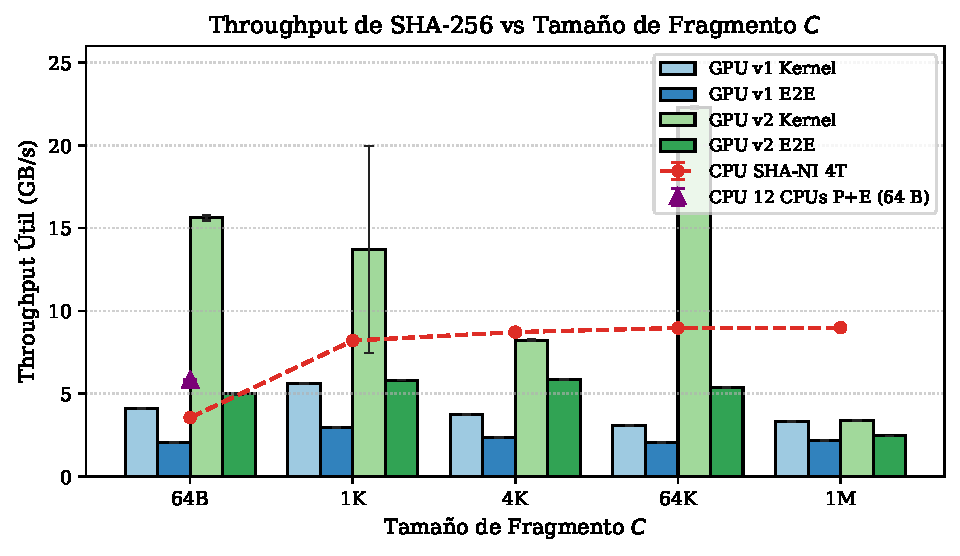
\includegraphics[width=\linewidth]{throughput_vs_c.pdf}
    \caption{Throughput de SHA-256 vs.~tamaño de fragmento $C$ para GPU v1/v2 (kernel-only y E2E, staging pinned) y serie de referencia CPU SHA-NI 4T evaluada a cada tamaño $C$, incorporando barras de error con la desviación estándar.}
    \label{fig:throughput_vs_c}
\end{figure}

Como sintetiza la Figura~\ref{fig:throughput_vs_c}, la GPU v2 supera a la CPU SHA-NI 4T en throughput E2E únicamente en el escenario de fragmentos mínimos $C=64$~B (\macrogputputeetwopinned~GB/s frente a \macrocputputfour~GB/s). Para todo $C \geq 1$~KB, la CPU SHA-NI 4T supera con claridad el rendimiento E2E de la GPU (alcanzando 8.21~GB/s en 1~KB y 8.99~GB/s en 1~MB), beneficiándose de operar en la memoria principal del host sin cruzar el enlace PCIe.

\subsection{Comparación CPU vs.~GPU}

La Tabla~\ref{tab:comparison} consolida las configuraciones evaluadas para el escenario principal $C=64$~B, destacando tres conclusiones principales:
\begin{itemize}
    \item \textbf{Rendimiento E2E y transferencia de bus:} En mensajes mínimos ($C=64$~B), la GPU v2 E2E con memoria pinned supera a la referencia CPU SHA-NI 4T. No obstante, al activar todos los núcleos disponibles de la CPU, tanto SHA-NI 8T como la configuración heterogénea 12 CPUs (P+E) bajo planificación dinámica revierten la ventaja y sobrepasan el throughput E2E de la GPU, al beneficiarse de acceso directo a la memoria principal del sistema sin sufrir la saturación del bus periférico PCIe.
    \item \textbf{Eficiencia energética de dispositivo vs. sistema completo:} Considerada como dispositivo aislado, la GPU en modo E2E consume menos energía neta por gigabyte que la referencia CPU SHA-NI 4T. Sin embargo, al incorporar el consumo activo del procesador anfitrión requerido para la gestión de buffers pinned y streams CUDA, la eficiencia integral se degrada; consecuentemente, la CPU SHA-NI 12 CPUs (P+E) se establece como la arquitectura globalmente más eficiente del sistema completo, además de entregar mayor throughput útil.
    \item \textbf{Potencial aritmético de cómputo puro:} En régimen kernel-only (datos residentes en VRAM), la GPU v2 demuestra una tasa de procesamiento muy superior a cualquiera de las configuraciones de CPU. Esta ventaja sugiere como hipótesis que la GPU resultaría intrínsecamente más eficiente energéticamente si las transferencias periféricas fuesen amortizadas por algoritmos criptográficos iterativos de múltiples rondas locales, mientras que para flujos de red o transacciones independientes de un solo paso, el bus PCIe determina el rendimiento final.
\end{itemize}

\begin{table}[htbp]
  \caption{Comparación cruzada de rendimiento y eficiencia energética ($C=64$~B)}
  \label{tab:comparison}
  \centering
  \setlength{\tabcolsep}{3.5pt}
  \resizebox{\columnwidth}{!}{%
  \begin{tabular}{lccccc}
    \toprule
    \textbf{Plataforma / Config.} & \textbf{Throughput (GB/s)} & \textbf{Mhash/s} & \textbf{J/GB neto (disp.)} & \textbf{J/GB neto (+host)} & \textbf{Speedup$^a$} \\
    \midrule
    Escalar 1T               & 0.11 $\pm$ 0.00      &   1.71 $\pm$ 0.00 & 45.58 $\pm$ 0.05 & 45.58 $\pm$ 0.05 & 0.03$\times$ \\
    SHA-NI 4T (ref.)         & 3.55 $\pm$ 0.00      &  55.45 $\pm$ 0.01 &  4.13 $\pm$ 0.05 &  4.13 $\pm$ 0.05 & 1.00$\times$ \\
    SHA-NI 8T                & 5.60 $\pm$ 0.02      &  87.45 $\pm$ 0.35 &  2.67 $\pm$ 0.05 &  2.67 $\pm$ 0.05 & 1.58$\times$ \\
    SHA-NI 12T (8E sob.)     & 5.62 $\pm$ 0.07      &  87.77 $\pm$ 1.06 &  2.69 $\pm$ 0.09 &  2.69 $\pm$ 0.09 & 1.58$\times$ \\
    SHA-NI 12 CPUs (P+E)     & 5.84 $\pm$ 0.02      &  91.25 $\pm$ 0.24 &  2.53 $\pm$ 0.02 &  2.53 $\pm$ 0.02 & 1.65$\times$ \\
    GPU v2 kernel            & 15.62 $\pm$ 0.15     & 244.02 $\pm$ 2.38 &  1.62 $\pm$ 0.02 &  2.45 $\pm$ 0.04 & 4.40$\times$ \\
    GPU v2 E2E pinned        & 4.98 $\pm$ 0.02      &  77.86 $\pm$ 0.33 &  3.49 $\pm$ 0.04 &  5.48 $\pm$ 0.07 & 1.40$\times$ \\
    \midrule
    FPGA (Spartan-7)         & \TODO{}             & \TODO{}          & \TODO{}         & \TODO{}         & \TODO{} \\
    \bottomrule
    \multicolumn{6}{l}{\footnotesize $^a$Speedup vs.~CPU SHA-NI 4T E2E ($C=64$~B). El speedup de GPU v2 kernel (aislado en VRAM) no es comparable con E2E.} \\
    \multicolumn{6}{l}{\footnotesize J/GB neto (+host) suma la energía RAPL PKG del host durante la ejecución (excluye DRAM en todas las plataformas).} \\
  \end{tabular}%
  }
\end{table}


%% ─────────────────────────────────────────────────────────────────
\subsection{Resultados de FPGA}
%% ─────────────────────────────────────────────────────────────────

La Tabla~\ref{tab:fpga} presentará los resultados post-implementación para el
acelerador SHA-256 RTL personalizado sintetizado en la FPGA AMD/Xilinx Spartan-7.

\begin{table}[htbp]
  \caption{Resultados del Acelerador RTL SHA-256 en FPGA (Xilinx Spartan-7)}
  \label{tab:fpga}
  \centering
  \begin{tabular}{lc}
    \toprule
    \textbf{Parámetro} & \textbf{Valor} \\
    \midrule
    Dispositivo Objetivo     & Xilinx Spartan-7 (xc7s50) \\
    HDL                      & Verilog RTL \\
    $f_{\max}$ (MHz)         & TBD \\
    Ciclos de Reloj / Bloque & TBD \\
    Throughput (Mbps)        & TBD \\
    Utilización de LUT       & TBD / 32{,}600 (TBD\%) \\
    Utilización de FF        & TBD / 65{,}200 (TBD\%) \\
    DSPs Usados              & TBD \\
    Potencia en el chip (W)  & TBD \\
    Eficiencia Energética (J/GB) & TBD \\
    Speedup vs.\ CPU SHA-NI 4T  & TBD \\
    \bottomrule
  \end{tabular}
\end{table}

La implementación FPGA se enfoca en maximizar la eficiencia energética mediante
control RTL determinista: la ruta de datos dedicada elimina la sobrecarga de
recuperación de instrucciones y el costo del predictor de saltos inherente a los
procesadores de propósito general, a la vez que evita el cuello de botella de la
transferencia PCIe que limita el throughput efectivo de la GPU.

\section{Conclusiones}
Este artículo evaluó empíricamente el algoritmo criptográfico SHA-256 bajo un marco heterogéneo comparando CPU con extensiones SHA-NI, GPU bajo modelo SIMT y FPGA personalizada en RTL, sobre un flujo masivo de mensajes independientes de 64~B. Las mediciones demuestran que, si bien la GPU ofrece un potencial aritmético masivo en cómputo puro en VRAM (15.62~GB/s), su tasa extremo a extremo queda estrangulada por el bus PCIe a 4.98~GB/s. En contrapartida, la CPU heterogénea asistida por planificación dinámica libre de cerrojos y operando sobre memoria local supera el throughput E2E de la GPU con 5.84~GB/s y consolida la mayor eficiencia energética global de sistema completo (2.53~J/GB netos con host frente a 5.48~J/GB de GPU+host). La caracterización final del acelerador RTL en FPGA permanece en curso (\TODO{integrar resultados finales post-implementación de throughput, potencia en chip y recursos LUT/FF/DSP en Spartan-7}), cuya incorporación consolidará la comparativa sistemática de tres vías.

\bibliographystyle{IEEEtran}
\bibliography{references}

\vspace{12pt}

\end{document}
